% ****** Start of file aipsamp.tex ******
%
%   This file is part of the AIP files in the AIP distribution for REVTeX 4.
%   Version 4.1 of REVTeX, October 2009
%
%   Copyright (c) 2009 American Institute of Physics.
%
%   See the AIP README file for restrictions and more information.
%
% TeX'ing this file requires that you have AMS-LaTeX 2.0 installed
% as well as the rest of the prerequisites for REVTeX 4.1
%
% It also requires running BibTeX. The commands are as follows:
%
%  1)  latex  aipsamp
%  2)  bibtex aipsamp
%  3)  latex  aipsamp
%  4)  latex  aipsamp
%
% Use this file as a source of example code for your aip document.
% Use the file aiptemplate.tex as a template for your document.
\documentclass[%
 aps,
 %jmp,%
 %prb,
 prl,
 amsmath,amssymb,
 %preprint,%
 %superscriptaddress,
 reprint,%
 %floatfix,
%author-year,%
%author-numerical,%
]{revtex4-1}
%]{article}

\usepackage{graphicx}% Include figure files
\usepackage{dcolumn}% Align table columns on decimal point
\usepackage{bm}% bold math
%\usepackage[mathlines]{lineno}% Enable numbering of text and display math
%\linenumbers\relax % Commence numbering lines

% Alter some LaTeX defaults for better treatment of figures:
    % See p.105 of "TeX Unbound" for suggested values.
    % See pp. 199-200 of Lamport's "LaTeX" book for details.
    %   General parameters, for ALL pages:
    \renewcommand{\topfraction}{0.9}    % max fraction of floats at top
    \renewcommand{\bottomfraction}{0.8}    % max fraction of floats at bottom
    %   Parameters for TEXT pages (not float pages):
    \setcounter{topnumber}{2}
    \setcounter{bottomnumber}{2}
    \setcounter{totalnumber}{4}     % 2 may work better
    \setcounter{dbltopnumber}{2}    % for 2-column pages
    \renewcommand{\dbltopfraction}{0.9}    % fit big float above 2-col. text
    \renewcommand{\textfraction}{0.07}    % allow minimal text w. figs
    %   Parameters for FLOAT pages (not text pages):
    \renewcommand{\floatpagefraction}{0.7}    % require fuller float pages
    % N.B.: floatpagefraction MUST be less than topfraction !!
    \renewcommand{\dblfloatpagefraction}{0.7}    % require fuller float pages
    % remember to use [htp] or [htpb] for placement

\begin{document}
%\title{Reduction of turbulent fluctuations and crossphase through driven sheared flow on the Large Plasma Device}
\title{Observation of improved and degraded confinement with driven flow on the LAPD}
\author{D.A. Schaffner}
\author{T.A Carter}
\author{G.D. Rossi}
\author{D.S. Guice}
\author{J. Maggs}
\author{S. Vincena}
\author{B. Friedman}
	\affiliation{Department of Physics and Astronomy, University of Los Angeles.}%Lines break automatically or can be forced with \\

\date{\today}% It is always \today, today,
             %  but any date may be explicitly specified

\begin{abstract}
Continuous control over the azimuthal flow and flow shear in the edge
region of the Large Plasma Device (LAPD) has been acheived using a
biasable limiter.  LAPD rotates spontaneously in the ion diamagnetic
direction (IDD); positive bias on the limiter allows this spontaneous
flow to be reduced, minimized (producing a near-zero flow and flow
shear state), and reversed to strong flow in the electron diamagnetic direction.  This new capability has enabled a
detailed study of the effect of flow shear on turbulence and transport
in LAPD.  In the minimum flow/shear state, confinement is degraded
relative to the spontaneously flowing LAPD edge:  the edge gradient scale
length increases as does fluctuation amplitude and turbulent particle
flux.  Particle flux and density fluctuations
are observed to decrease with increasing shearing rate, with
substantial reduction (BE QUANTITATIVE HERE) with shearing rate equal
to the zero-flow turbulent autocorrelation time.  This
variation is largely insensitive to the direction of the flow; the
transport depends primarily on the magnitude of the shearing rate. 
Measurements of density-potential crossphase and coherency show
that low frequency ($<10$kHz) flux suppression is dominated by
decreased density fluctuation amplitude while high frequency ($>10$kHz) flux reduction
is dominated by variation in the crossphase. Coherency between density and
electric field fluctuations also contributes to the observed reduction
in flux.  Electric field fluctuation amplitude appears to be mostly unaffected
by the variation shearing rate. Cross-correlation measurements show a reduction in
the radial correlation length with shear as well as enhanced
correlation length in the azimuthal direction.   The variations of
flux, density fluctuation amplitude, crossphase and radial correlation
length with shearing rate are fit well with power laws.


%% Shearing rates up to five times the (no flow) turbulent
%% decorrelation rate are achieved. 
%% Density profiles show degraded confinement in the low shear state and improved confinement in the higher shearing states in both flow directions characterized by a gradual transition. Gradient scale lengths range from 15cm at no shear to 9cm in IDD flow shear and 4cm in EDD flow shear. Radially outward particle flux decreases with shear. Measurements of turbulent fluctuations crossphase, and coherency show that low frequency ($<10$kHz) flux suppression is dominated by density fluctuations decreases while high frequency ($>10$kHz)flux suppression is dominated  density/E-field crossphase decreases as turbulent fluctuations increase in this regime. Coherency between isat and E-field fluctuations also appears to be a contributer to flux suppresion, though electric field power appear to be mostly uneffected by shearing rate. Cross-correlation measurements show a reduction in the radial correlation length with shear as well as enhanced correlation length in the azimuthal direction and some eddy-tilting depending on flow direction. Flux, fluctuations, crossphase and radial correlation length can all be fit to power-laws consistent with theory prediction.

Recent biasing experiments on the Large Plasma Device (LAPD) have allowed for a fine variation of azimuthal flow shear states from spontaneous flow in the ion diamagnetic direction (IDD) to a zero flow state, to a large flow and shear state in the electron diamagnetic direction (EDD). Shearing rates up to five times the turbulent decorrelation rate are achieved. Density profiles show degraded confinement in the low shear state and improved confinement in the higher shearing states in both flow directions characterized by a gradual transition. Gradient scale lengths range from 15cm at no shear to 9cm in IDD flow shear and 4cm in EDD flow shear. Radially outward particle flux decreases with shear. Measurements of turbulent fluctuations crossphase, and coherency show that low frequency ($<10$kHz) flux suppression is dominated by density fluctuations decreases while high frequency ($>10$kHz)flux suppression is dominated  density/E-field crossphase decreases as turbulent fluctuations increase in this regime. Coherency between isat and E-field fluctuations also appears to be a contributer to flux suppresion, though electric field power appear to be mostly uneffected by shearing rate. Cross-correlation measurements show a reduction in the radial correlation length with shear as well as enhanced correlation length in the azimuthal direction and some eddy-tilting depending on flow direction. Flux, fluctuations, crossphase and radial correlation length can all be fit to power-laws consistent with theory prediction.
\end{abstract}

\maketitle
%\section{Introduction}  No need for section titles in PRL, save space

%% Need to start with discussion of H-mode, role of flow.  Cite BDT, recent reviews of flow-shear interaction (Terry, Diamond, Tynan).  Move immediately to set up why this study is unique

The effect of flow and flow shear on plasma turbulence has long been studied as a mechanism for turbulence reduction and increased particle confinement in both tokamaks and linear machines.  The most dramatic observed effect of cross-field flow is the creation of a higher confinement state, called an H-mode, which has been first observed on the Continuous Current Tokamak (CCT) and in other tokamaks such as DII-D. While some plasma machines rely on a spontaneous flow to create sheared flow for study, other machines (TEXTOR, LAPD) have developed external biasing mechanisms to produce radial electric fields which can drive controllable azimuthal flow by $E \times B$ drift on many machines including TEXTOR \cite{boedo00}.

Theoretical investigation into the nature of effect of sheared flow has focused mainly on its influence on turbulent fluctuations \cite{biglari90} and on the crossphase between electric field and any advected quantity, such as density in the case of particle flux \cite{ware96,terry01}. Fluctuation reduction due to shear comes from the reduction in radial correlation length---due to the shearing of turbulent eddies---while the effect of crossphase has to do with the fact that turbulent particle flux relies on the phasing of outward or inward ExB flows with increases in density. The simplest mode non-specific models for the effect of shearing on turbulent fluctuations predict a power law decrease\cite{biglari90}, while crossphase can have an even stronger scaling\cite{terry01}.

The experiment in this letter is an extension of previous biasing experiments on LAPD. In one, an inward pointing electric field produced by chamber biasing demonstrated that increased flow shear resulted in turbulent modification and increased particle confinement\cite{carter09}. However, penetration of the electric field was low until high biases resulting in sudden transition from background states to confined states. In another experiment, it was shown that a small biased annulus could produce sheared flows within the main column of the plasma\cite{zhou12}. In this letter, a new biasing mechanism has allowed for smooth transition from a low flow shear state-LAPD's natural state-to zero shear state, to a high shear state. With this smooth control of flow shear, we can carefully observe the effect of shear on turbulent fluctuations, particle flux, and gradient length scale to a level of detail that allows for comparison to theory prediction.

In this letter, we report on the observation of a degraded and enhanced confinement state as a function of a fine variation of driven sheared-flows up to five times a no-shear turbulent decorrelation rate and that this confinement occurs regardless of flow or flow shear direction. We have shown that this variation in confinement correlates with increases and decreases in particle flux. Moreover, we can show that radial correlation length, particle flux, crossphase, density fluctuations all decrease with shearing rate and that substantial decreases begin with rates as small as one-half the turbulent decorrelation rate. We observe differing characteristics depending on which frequency regime in examined. Namely, we see that suppression of flux at frequencies less than 10kHz are dominated by decreases in density fluctuations while flux suppression at greater than 10kHz is dominated by crossphase and coherency decreases. Lastly, we note that electric field fluctuations appear to be minamally affected by shearing changes. Given the ability to scan from a non-sheared state to a highly sheared state, we can fit the various quantities to a power-law decay as predicted by theory \cite{biglari90}.

The Large Plasma Device \cite{gek91} (LAPD) is a 20m by 1m cylindrical linear device with a 54cm wide barium-oxide coated nickel cathode pulsed at 1Hz to produce a 45eV electron beam which ionizes the helium gas in the chamber. A column long plasma of density about $5 \times 10^{12}$ cm$^{3}$ and temperature of 5eV is produced. The field for this experiment was set to 1000G. To produce the bias, four quarter annulus aluminum plates are inserted half a meter beyond the cathode creating a flat boundary condition from the chamber wall to the opening of a 25cm aperture. A pulse power circuit connected to a capacitor bank supplies a 5ms bias during the 15ms plasma discharge with a voltage range from floating potential to 230V. Measurements of saturated current and floating potential are taken with a 9-tip flush surface tantalum probe while temperature and plasma potential is taken by swept Langmuir probe.

Azimuthal flow and flow shear are controlled by adjusting the voltage on the capacitor bank which produces a voltage on the limiter places. When voltages of the limiter on are approximately less than the voltage of the anode (between floating potential of about 35V to about 45V with respect to chamber ground), an overall azimuthal flow occurs in the ion diamagnetic direction shown in
Fig.~\ref{fig:velocity_flowshear}
with velocities peaking just outside the limiter edge. When the voltage on the limiter is brought near anode potential, flow and flow shear zero out. Voltages above anode produce electron diamagnetic direction flows peaked at the limiter edge. The voltage on the power supply cannot be set below the floating potential as the plasma tends to charge the capacitor banks.

Measurements of saturated current and particle flux are taken for each bias flow state. A set of radial values are averaged over a range from 27 to 31cm in a region where such averaged flow and flow shear scale approximately linearly with limiter bias as in 
Fig.~\ref{fig:velocity_flowshear}%
and are outside the limiter edge to avoid any possible effects from fast electrons. Maxing out at about 125kHz, we can achieve a shearing rate of approimately five times the natural turbulent decorrelation rate. The no flow, no shear regime allows us to directly measure a turbulent decorrelation rate. An autocorrelation time of about 36us is calculated by taking the full width at half max of a Hilbert transform of the isat autocorrelation function at the no flow/shear bias yielding a decorrelation rate of $\Delta \omega_{t} = $ 28kHz.

Calculated quantites are used to characterize flux and length scale. Density gradient length scale is calculated by $L_{\xi} = \lvert \nabla \ln \xi \rvert ^{-1}$ while particle flux, $\Gamma_{p} = \langle \tilde{n} \tilde{v_{r}} \rangle = \langle \tilde{n} \tilde{E_{\theta}} \rangle /B$, can be calculated spectrally as
\begin{equation}
\Gamma_{p} = \frac{2}{B} \int^{\infty}_{0} \lvert n(\omega) \rvert \lvert E_{\theta}(\omega) \rvert \gamma_{n,E_{\theta}}(\omega) \cos [\phi_{n,E_{\theta}}(\omega)] d\omega.
\label{eq:fluxint}
\end{equation}
which also allows us to directly determine the contributions of turublent fluctuations, crossphase and coherency to the particle flux.

%\section{Theory and Background}
%  Don't need this, instead add to intro in shortened form

%The primary goal of this experiment is to observe the effect of sheared flow on radial particle confinement and turbulence in general. %The main avenues of investigation are through a global measurement of radial density profiles which can qualitatively demonstrate %relative particle confinement and through the local particle flux, $\Gamma_{p}$, a calculated value taken from direct time-series %measurements of density and electric field using 
%\begin{equation}
%\Gamma_{p} = \langle \tilde{n} \tilde{v_{r}} \rangle = \langle \tilde{n} \tilde{E_{\theta}} \rangle /B
%\label{eq:flux}
%\end{equation}
%where $r$ is the radial and $\theta$ is the azimuthal direction. Embedded in the flux information is both fluctuating power-both density %and electric field-as well as the relative phase between these two quantities: 
%\begin{equation}
%\Gamma_{p} = \frac{2}{B} \int^{\infty}_{0} \lvert n(\omega) \rvert \lvert E_{\theta}(\omega) \rvert \gamma_{n,E_{\theta}}(\omega) \cos %[\phi_{n,E_{\theta}}(\omega)] d\omega.
%\label{eq:fluxint}
%\end{equation}

\begin{figure}
\begin{center}
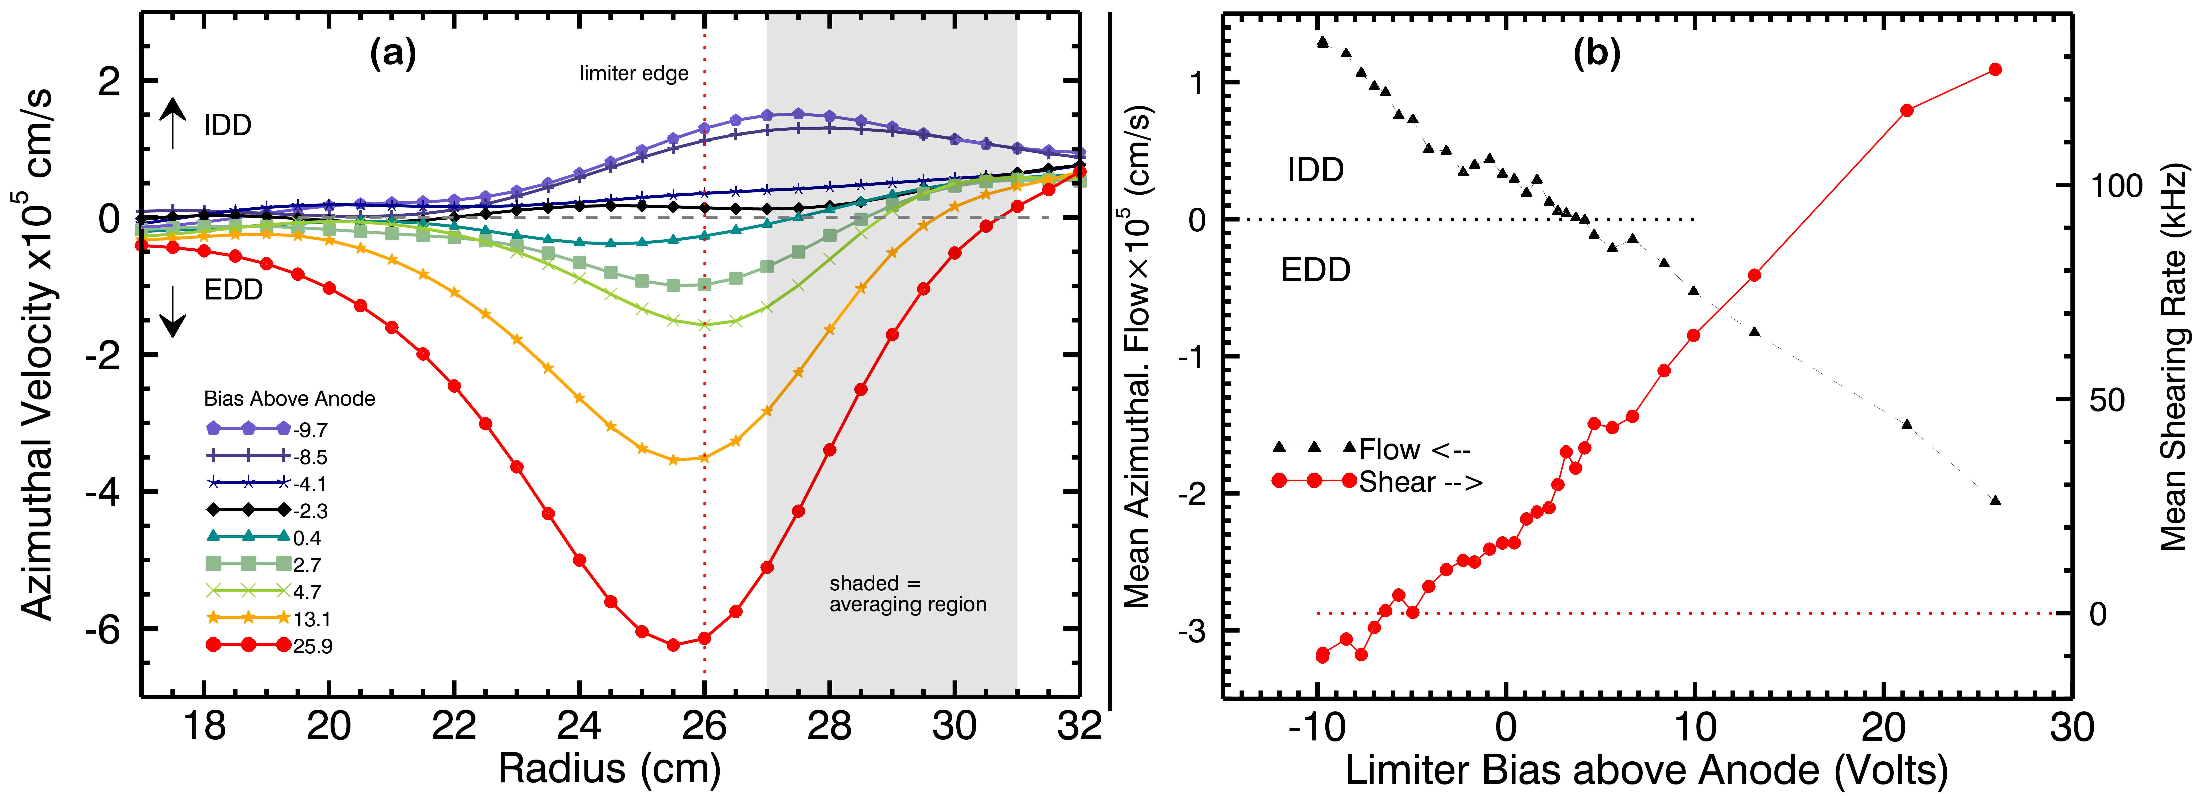
\includegraphics[width=8.5cm]{velocity_flowshear.pdf}% Here is how to import EPS art
%\includegraphics{figure1_velo}
\end{center}
\caption{\label{fig:velocity_flowshear} (a) Velocity profiles using plasma potential from swept measurements. (b) Nearly linear scaling of flow (black) and shearing (red) versus limiter bias.}
\end{figure}

%\begin{figure}
%\begin{center}
%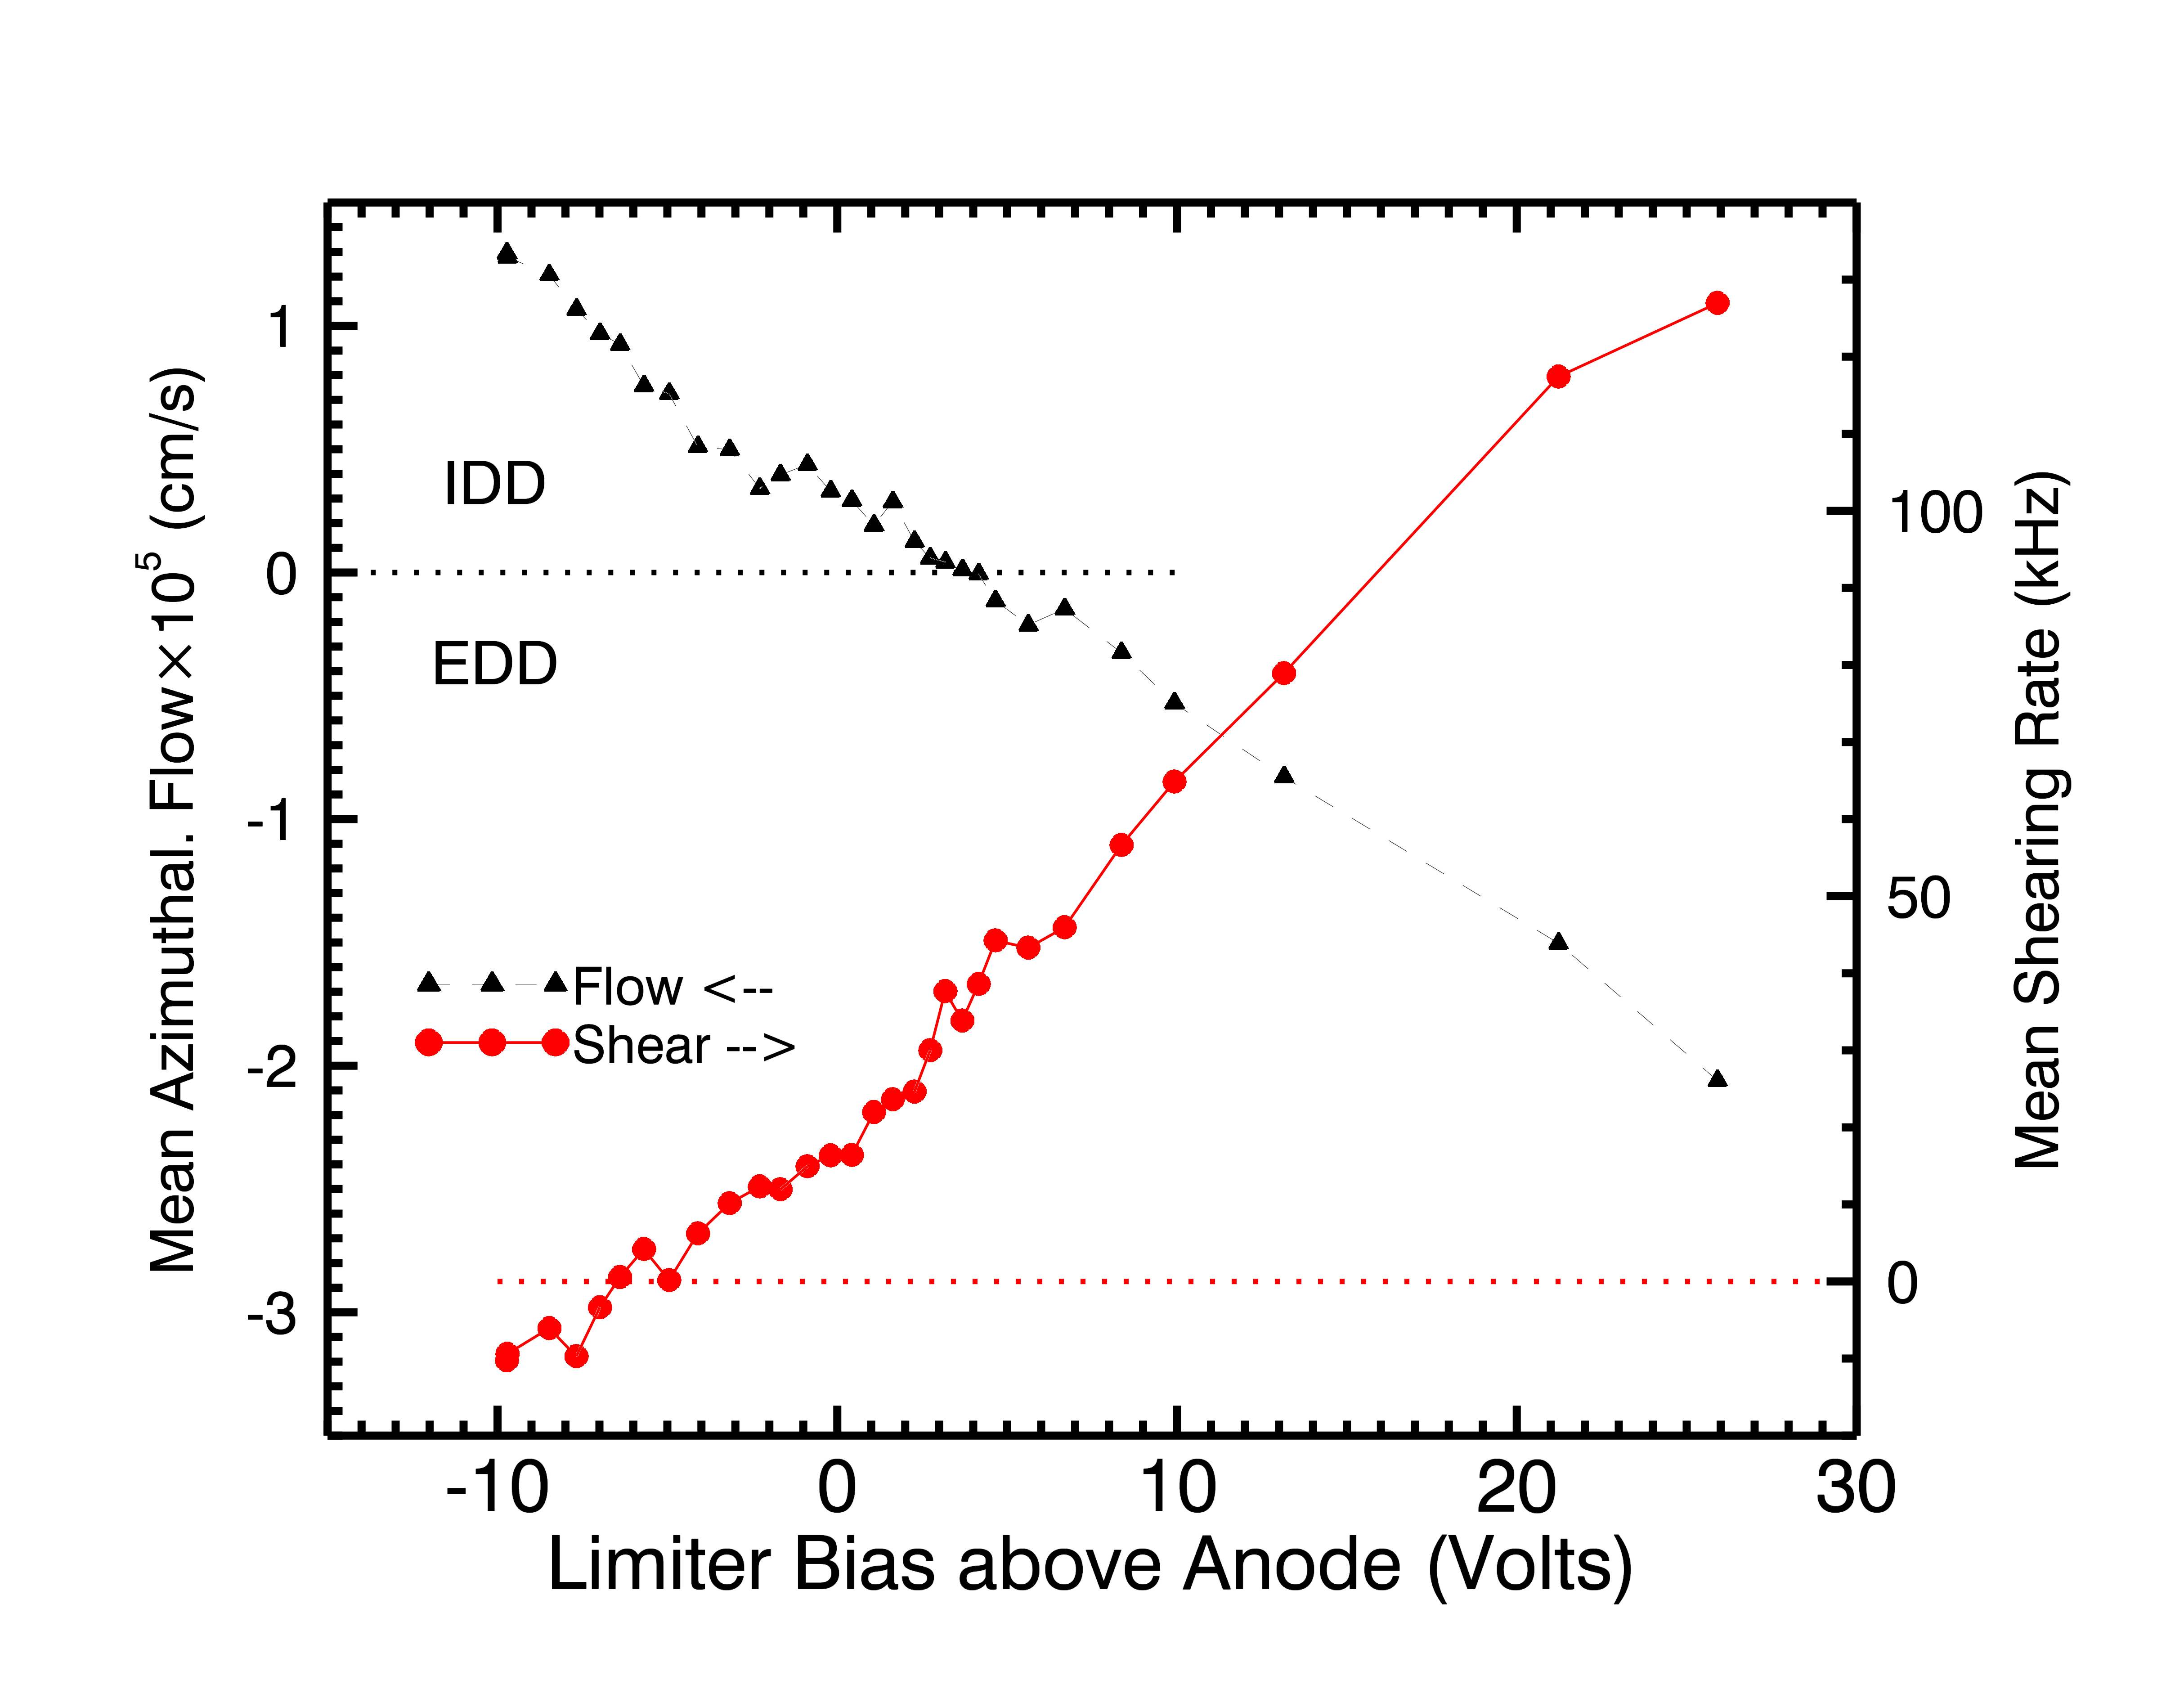
\includegraphics[width=8cm]{flowandshear.png}% Here is how to import EPS art
%\end{center}
%\caption{\label{fig:flowandshear} Nearly linear scaling of flow (black) and shearing (red) versus limiter bias.}
%\end{figure}

%To get a quantitative relationship between shearing rate and fluctuation power, an heuristic argument can be made \cite{biglari90} based %on turbulent fluctuation drive due to free energy from a gradient and decay from turbulent decorrelation for any fluctuating quantity %$\xi$, so that for stationary turbulence,
%\begin{equation}
%\tau_{f}^{-1} \langle \lvert \tilde{\xi}/\xi_{0} \rvert ^{2} \rangle = D/L_{\xi}^{2}
%\label{eq:flucsbalance}
%\end{equation}
%where $\tau_{f}$ is a general turbulent decorrelation timescale and $L_{\xi} = \lvert \nabla \ln \xi \rvert ^{-1}$ is the gradient scale %length and $D$ is the diffusivity. At zero shearing, $\tau_{f}$ is proportional to the standard mixing length $D/\Delta r^{2}$ where %$\Delta r$ is the radial correlation length. At strong shearing however, it can be shown that $\tau_{f}^{-1} = (\omega_{s}^{2} \Delta %\omega_{t})^{1/3}$ where $\omega_{s}$ is the shearing rate and $\Delta \omega_{t}$ is the turbulent decorrelation rate for zero %shearing. Thus flucuation power normalized to zero-shearing power scales to shearing rate as
%\begin{equation}
%\frac{\langle \lvert \tilde{\xi}/\xi_{0} \rvert ^{2} \rangle _{\omega_{s}}}{\langle \lvert \tilde{\xi}/\xi_{0} \rvert ^{2} \rangle %_{\omega_{s}=0}} = \left(\frac{\omega_{s}}{{\Delta \omega_{t}}}\right)^{-2/3}.
%\label{eq:flucsvsshear}
%\end{equation}

%Further calculations by Terry have suggested that the crossphase may be even more sensitive to shearing rate---up to two powers stronger %\cite{terry01}. Based on crossphase reduction, it is even conceivable to observe an overall reduction in flux despite no change or even %an increase in turbulent fluctuations.

The first clear observation shown in
Fig.~\ref{fig:densgrad}
\begin{center}
\begin{figure}
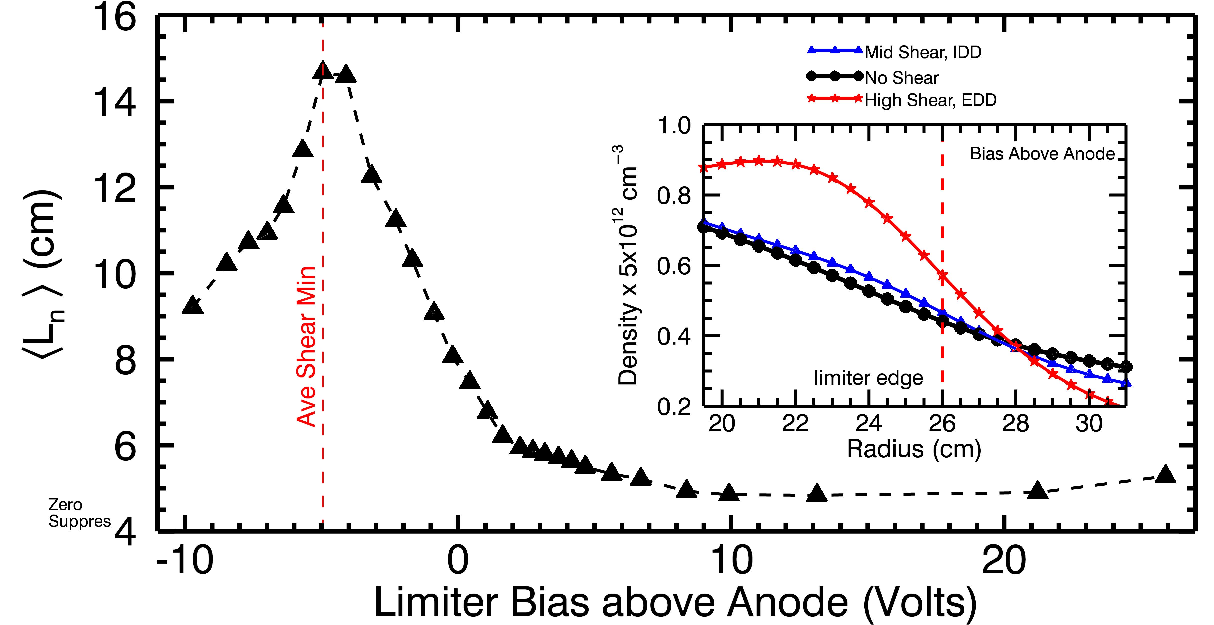
\includegraphics[width=8.5cm]{densgrad.pdf}% Here is how to import EPS art
\caption{\label{fig:densgrad} Density gradient length scale versus limiter bias. Inset shows density profile relaxing then steepening again with bias.}
\end{figure}
\end{center}
is a change in particle confinement level as bias is varied, as indicated by a change in the gradient scale length of the density radial profiles. The average density gradient scale length begins at 9cm with no bias, but as the limiter voltage increase to the point of minimum shearing rate, the density gradient levels out, reaching a scale length peak of about 15cm. As bias and shearing continue to increase, the density gradient steepens again fairly symmetrical about the shear minimum. Pushing the voltage higher causes the density gradient to steepen further reaching a saturated value of about 5cm. The initial scale length value and saturated values are consistent with previous biasing experiments done on the LAPD\cite{carter09}, but rather than see a density gradient degradation, a sharp threshold is observed. It is likely the new biasing setup allows this transition to be observed. It was spectulaed in the previous experiment that a threshold was observed not because of an inherent dependence on a shear value, but because of penetration of cross-field current---and thus flow---from the chamber edge to the plasma source. By placing the source of biasing current, the limiters, closer to the cathode edge, we can establish cross-field currents at lower shear values than before.

It should also be noted that the symmetry of the gradient scale length curve about the shear minimum is an indication that both IDD or EDD flow and shearing direction can produce a steepened density gradient. This is clearly seen in
Fig.~\ref{fig:shearandgrad}
\begin{figure}
\begin{center}
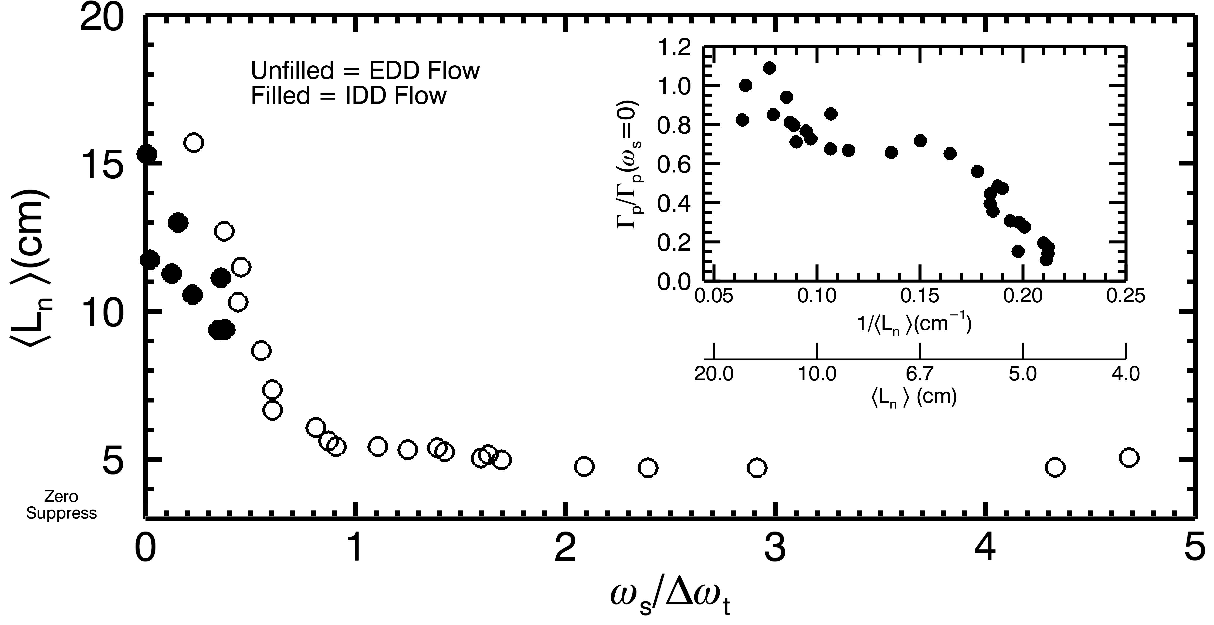
\includegraphics[width=8.5cm]{shearandgrad.pdf}% Here is how to import EPS art
\end{center}
\caption{\label{fig:shearandgrad} Gradient scale length versus shearing rate. Inset shows correlation of gradient scale length and turbulent particle flux.}
\end{figure}
with average gradient scale length compared to the ratio of shearing rate to decorrelation rate. Both IDD and EDD flow and flow shear points lie on the same curve.

The change in confinement can be connected to a change in the turbulence properties of the plasma which dictate the turbulent flux. An overview of fluctuation power in saturated current (as a proxy for density) can be seen in 
Fig.~\ref{fig:powercontour}
\begin{figure}
\begin{center}
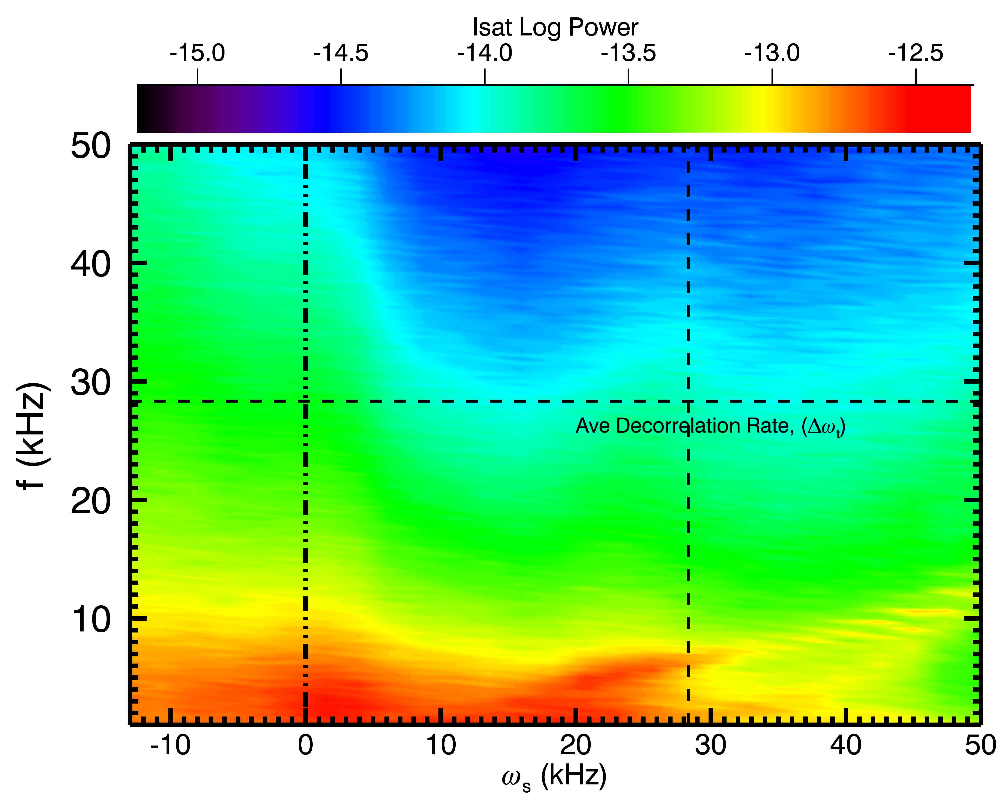
\includegraphics[width=8.5cm]{powercontour.pdf}% Here is how to import EPS art
\end{center}
\caption{\label{fig:powercontour} Contour plot of log isat fluctuation power versus shearing rate and frequency. Dashed lines show location of decorrelation rate.}
\end{figure}
where the power as a function of frequency has been scaled to the turbulent decorrelation rate. The contour plot shows that most of the turbulent power is less than 10kHz and that power decreases overall with increasing shearing rate. There does, however, appear to be a coherent mode growing when the shearing rate begins to match the turbulent decorrelation rate. 

The changes in gradient scale length are indicative of an overall change in particle flux. This flux can be directly measured by correlating fluctuating saturated current (as a proxy for density) with fluctuating radial flow---$E \times B$ flow using an electric field derived from two floating potential tips on either side of the density measuring saturated current tip. This flux can be rewritten in terms of an integral over fluctuation power, coherency and crossphase allowing separate comparison of the effect of shearing on turbulent power or crossphase. In addition to separating the contributions of fluctuation power and crossphase to the flux, the flux can be calculated over a certain frequency range. Like gradient scale length, normalized average particle flux decreases with shearing rate scaled to the turbulent decorrelation rate as in 
Fig.~\ref{fig:fluxvsshear}. 
\begin{figure}
\begin{center}
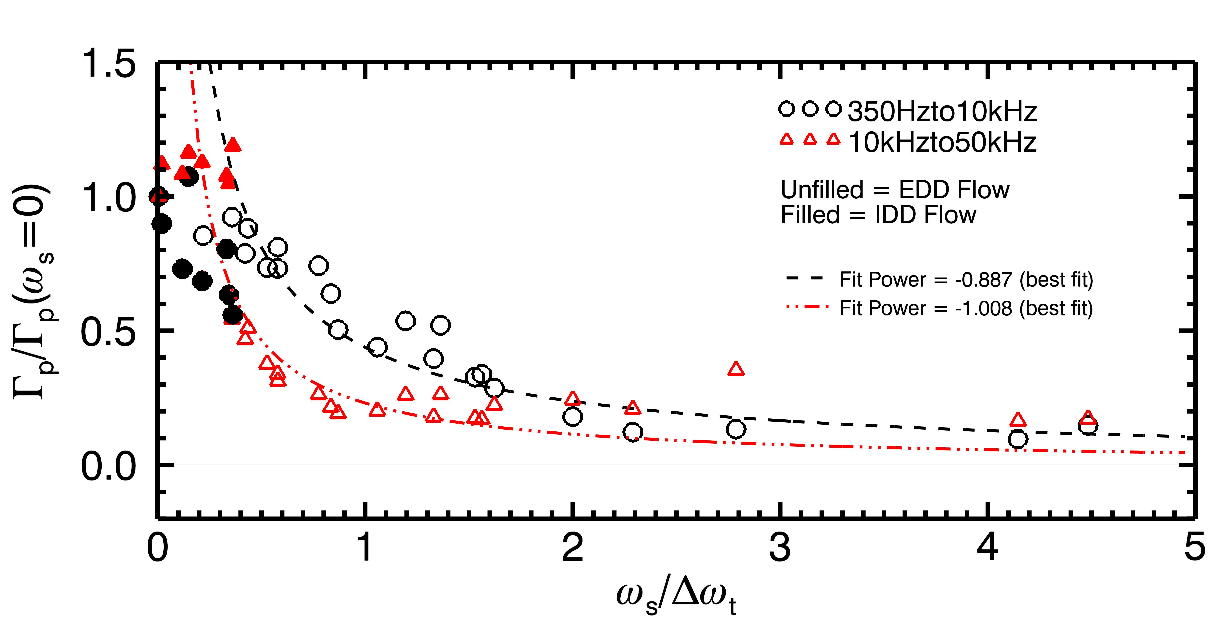
\includegraphics[width=8.5cm]{fluxvsshear.pdf}% Here is how to import EPS art
\end{center}
\caption{\label{fig:fluxvsshear} Particle flux as a function of shearing rate normalized to decorrelation rate. Black points show low frequency, red shows high. Filled symbols represent points with flow in IDD.}
\end{figure}
However, a clear difference emerges when the flux is bandwidth limited. The flux from 350Hz to 10kHz, where most of the fluctuation power is located, drops off gradually, hitting its minimum only at a shearing rate about three times the decorrelation rate. Higher bandwidth though, 10kHz to 50kHz, drops off much more quickly, nearing its minimum when shearing equals decorrelation rate. Best fit lines from log-log plots of these scatters using a power law form of $\left(\omega_{s}/\Delta \omega_{t}\right)^{\alpha}$ yield exponents of $\alpha = -0.887$ for the low bandwidth flux and about $\alpha = -1.008$ for the high bandwidth flux. 

The reason for the difference becomes evident when the flux is examined by its separate components as in 
Fig.~\ref{fig:fluxcomps}
\begin{figure}
\begin{center}
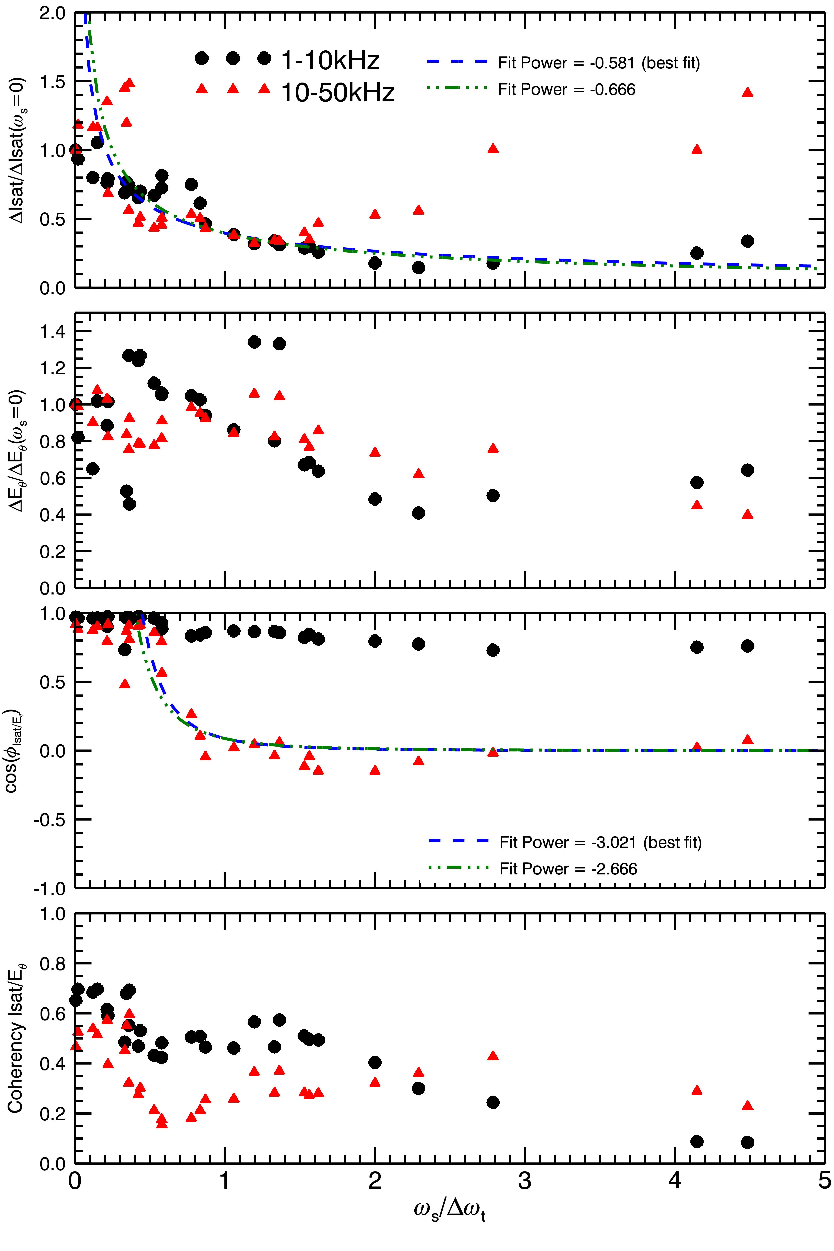
\includegraphics[width=8.5cm]{fluxcomps.pdf}% Here is how to import EPS art
\end{center}
\caption{\label{fig:fluxcomps} Components of particle flux versus shearing rate including isat/Density fluctuation power(a), electric field fluctuation power(b), crossphase(c) and coherency(d) with black points for low frequency, red for high.}
\end{figure}
. The top two plots show fluctuations power---saturated current and electric field---as functions of normalized shearing rate, while the bottom two show crossphase and coherency respectively. Observing the low bandwidth flux, isat power decreases gradually, with a power fit of $\alpha = 0.581$. Crossphase, on the other hand, does not decrease. In this bandwidth then, decreases in flux are primarily due to decreasing turbulent power. For high bandwidth flux, though, the opposite appears to be true. While isat fluctuations do decrease initially, they actually begin to increase at high shearing rates. In this case, the decrease in flux is primarily due to drops in crossphase and to some extent coherency, even despite an increase in isat turbulence. A fits to this high frequency crossphase calculation are yields $\alpha = -3.021$.  Electric field fluctuations, meanwhile, appear to not be substantially affected by shearing. For both high and low frequency, the fluctuation power is reduced by no more than 50\% with even the highest shearing achieved. For comparison to BDT theory, a curve of power $\alpha = -(2/3)$ is plotted for isat fluctuations, while a curve of power $\alpha = -(8/3)$, two powers larger than $-(2/3)$, is show for the crossphase plot.

%The frequency dependence on flux is even more evident in
%Fig.~\ref{fig:powercontour}
%\begin{figure}
%\begin{center}
%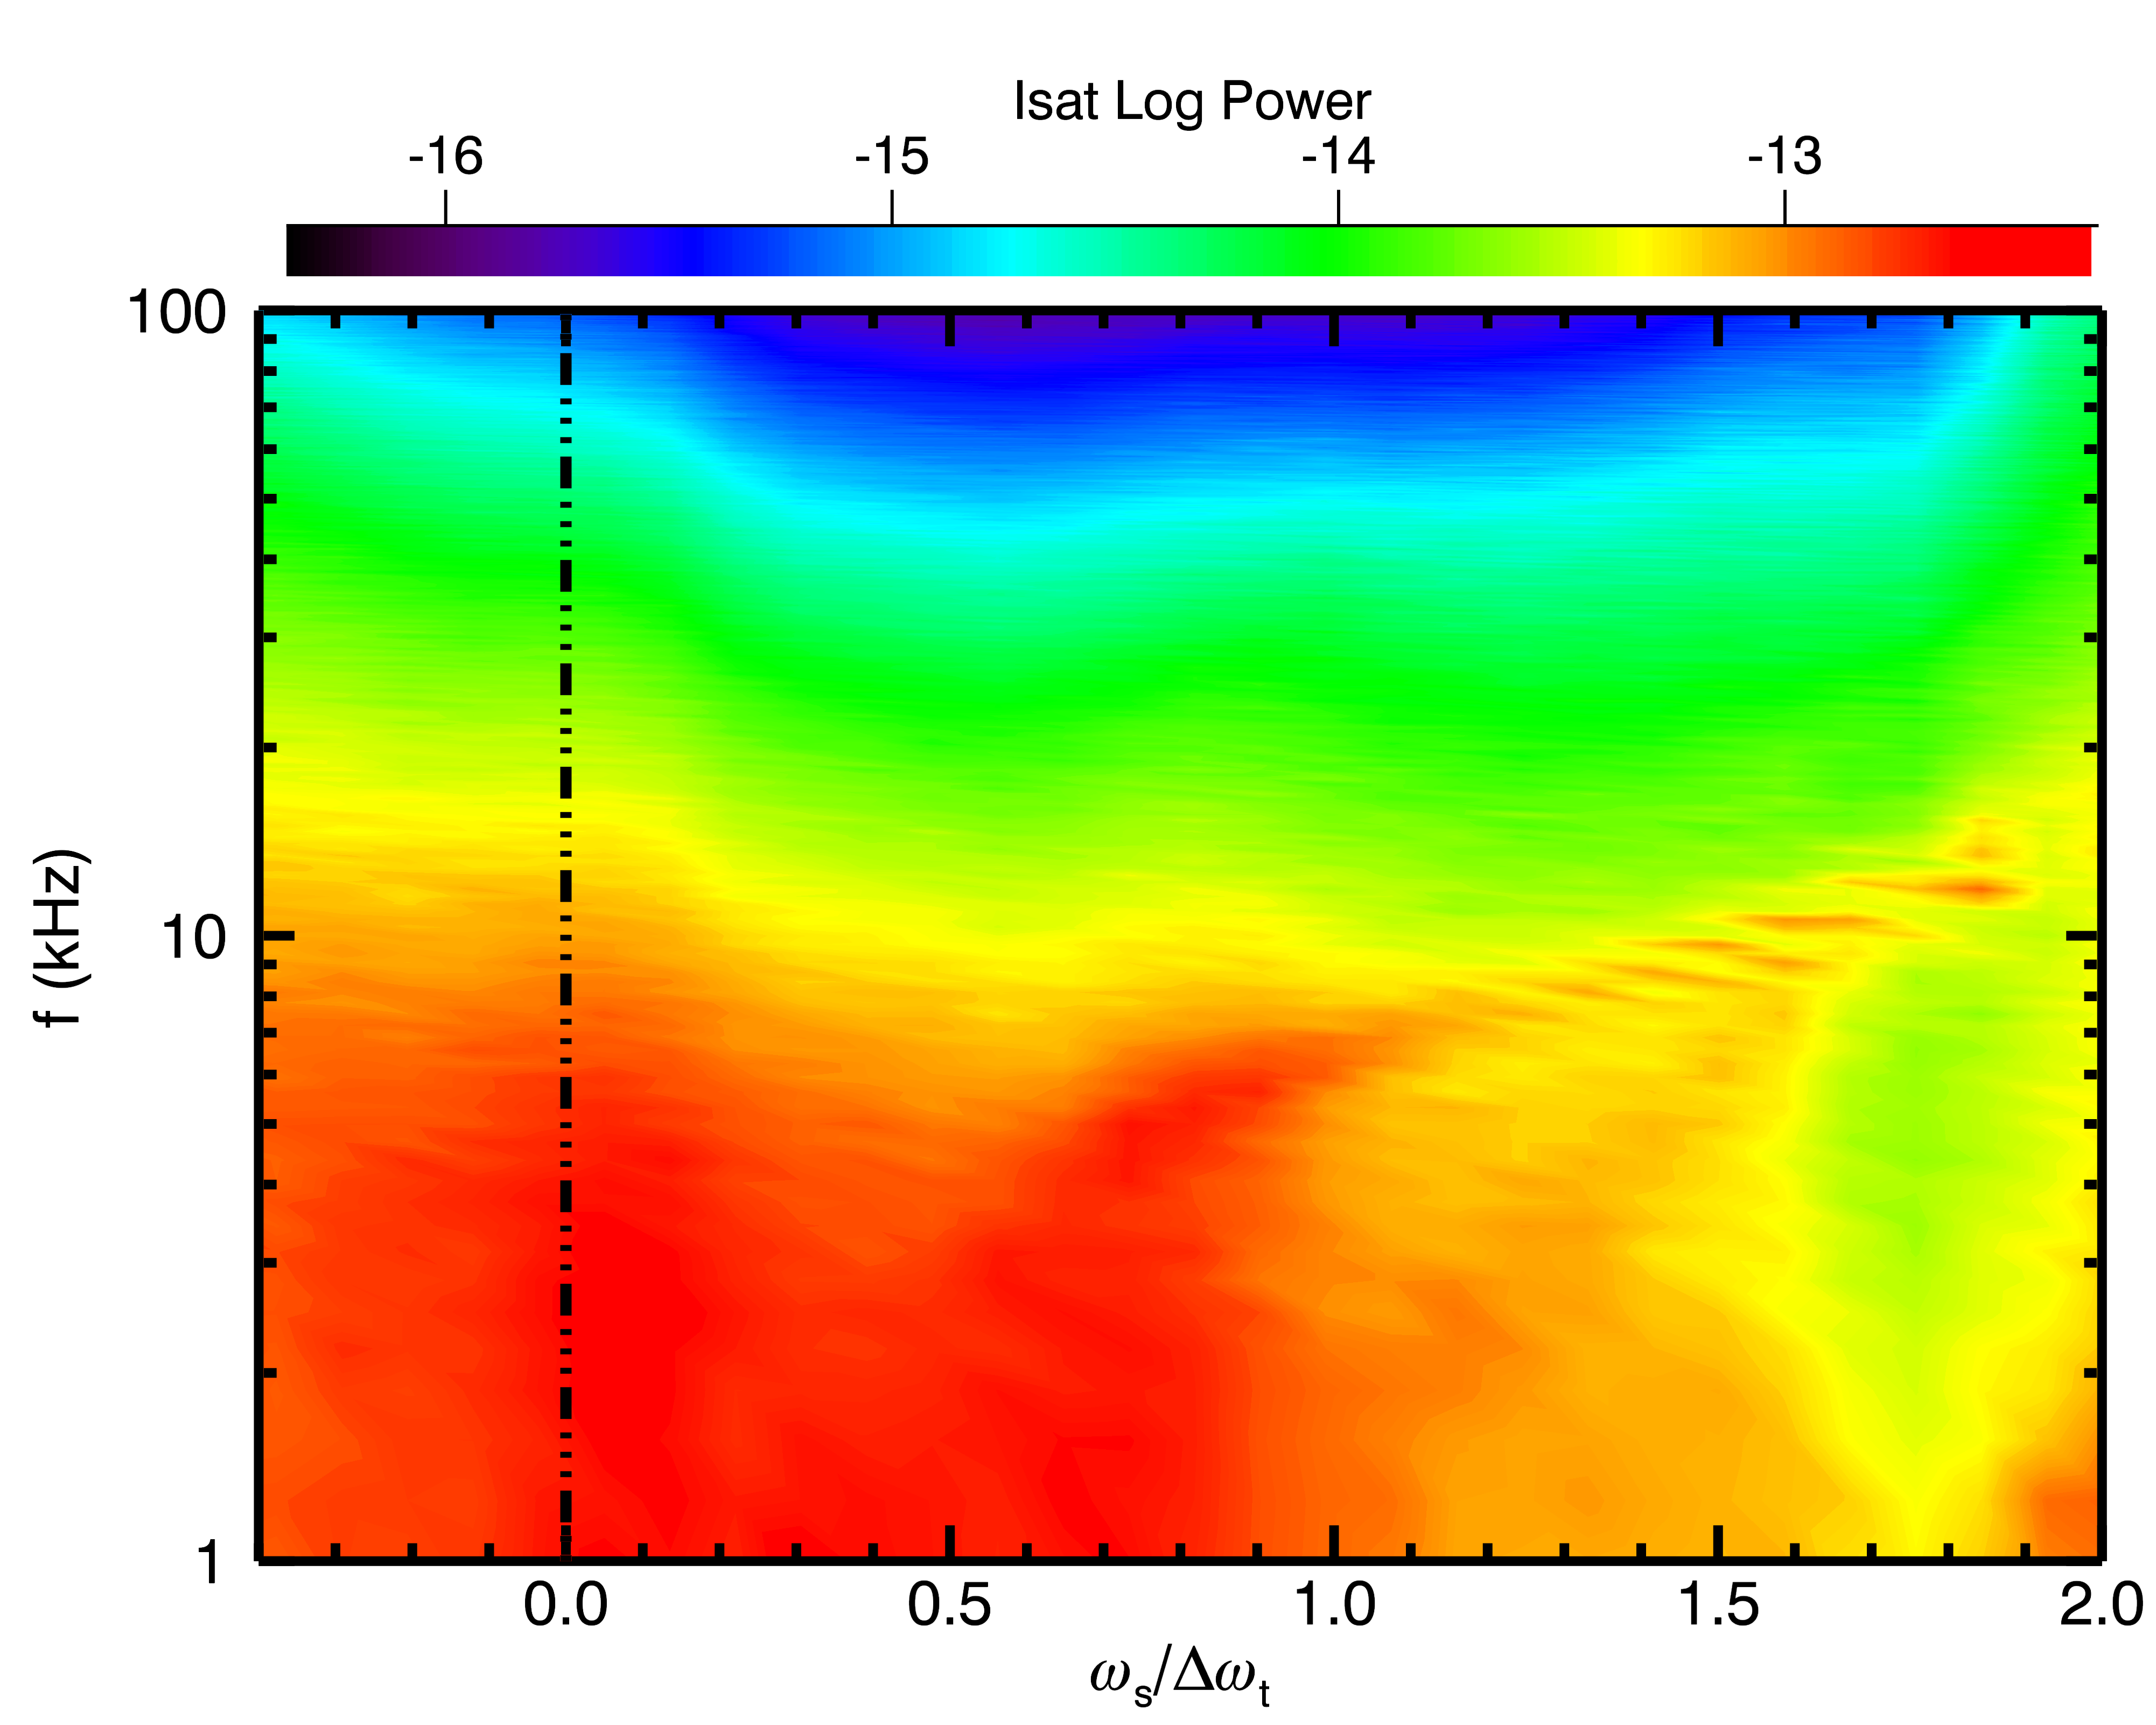
\includegraphics[width=8cm]{powercontour.png}% Here is how to import EPS art
%\end{center}
%\caption{\label{fig:powercontour} Contour plot of log isat fluctuation power versus shearing rate and frequency. Dashed lines show %location of decorrelation rate.}
%\end{figure}
%showing a contour map of fluctuation power or crossphase versus frequency and shearing rate. Isat power peaks at zero shearing rate and %tends to decrease gradually for all frequencies up to about 20kHz. Crossphase however 
%Fig.~\ref{fig:cpcontour}
%\begin{figure}
%\begin{center}
%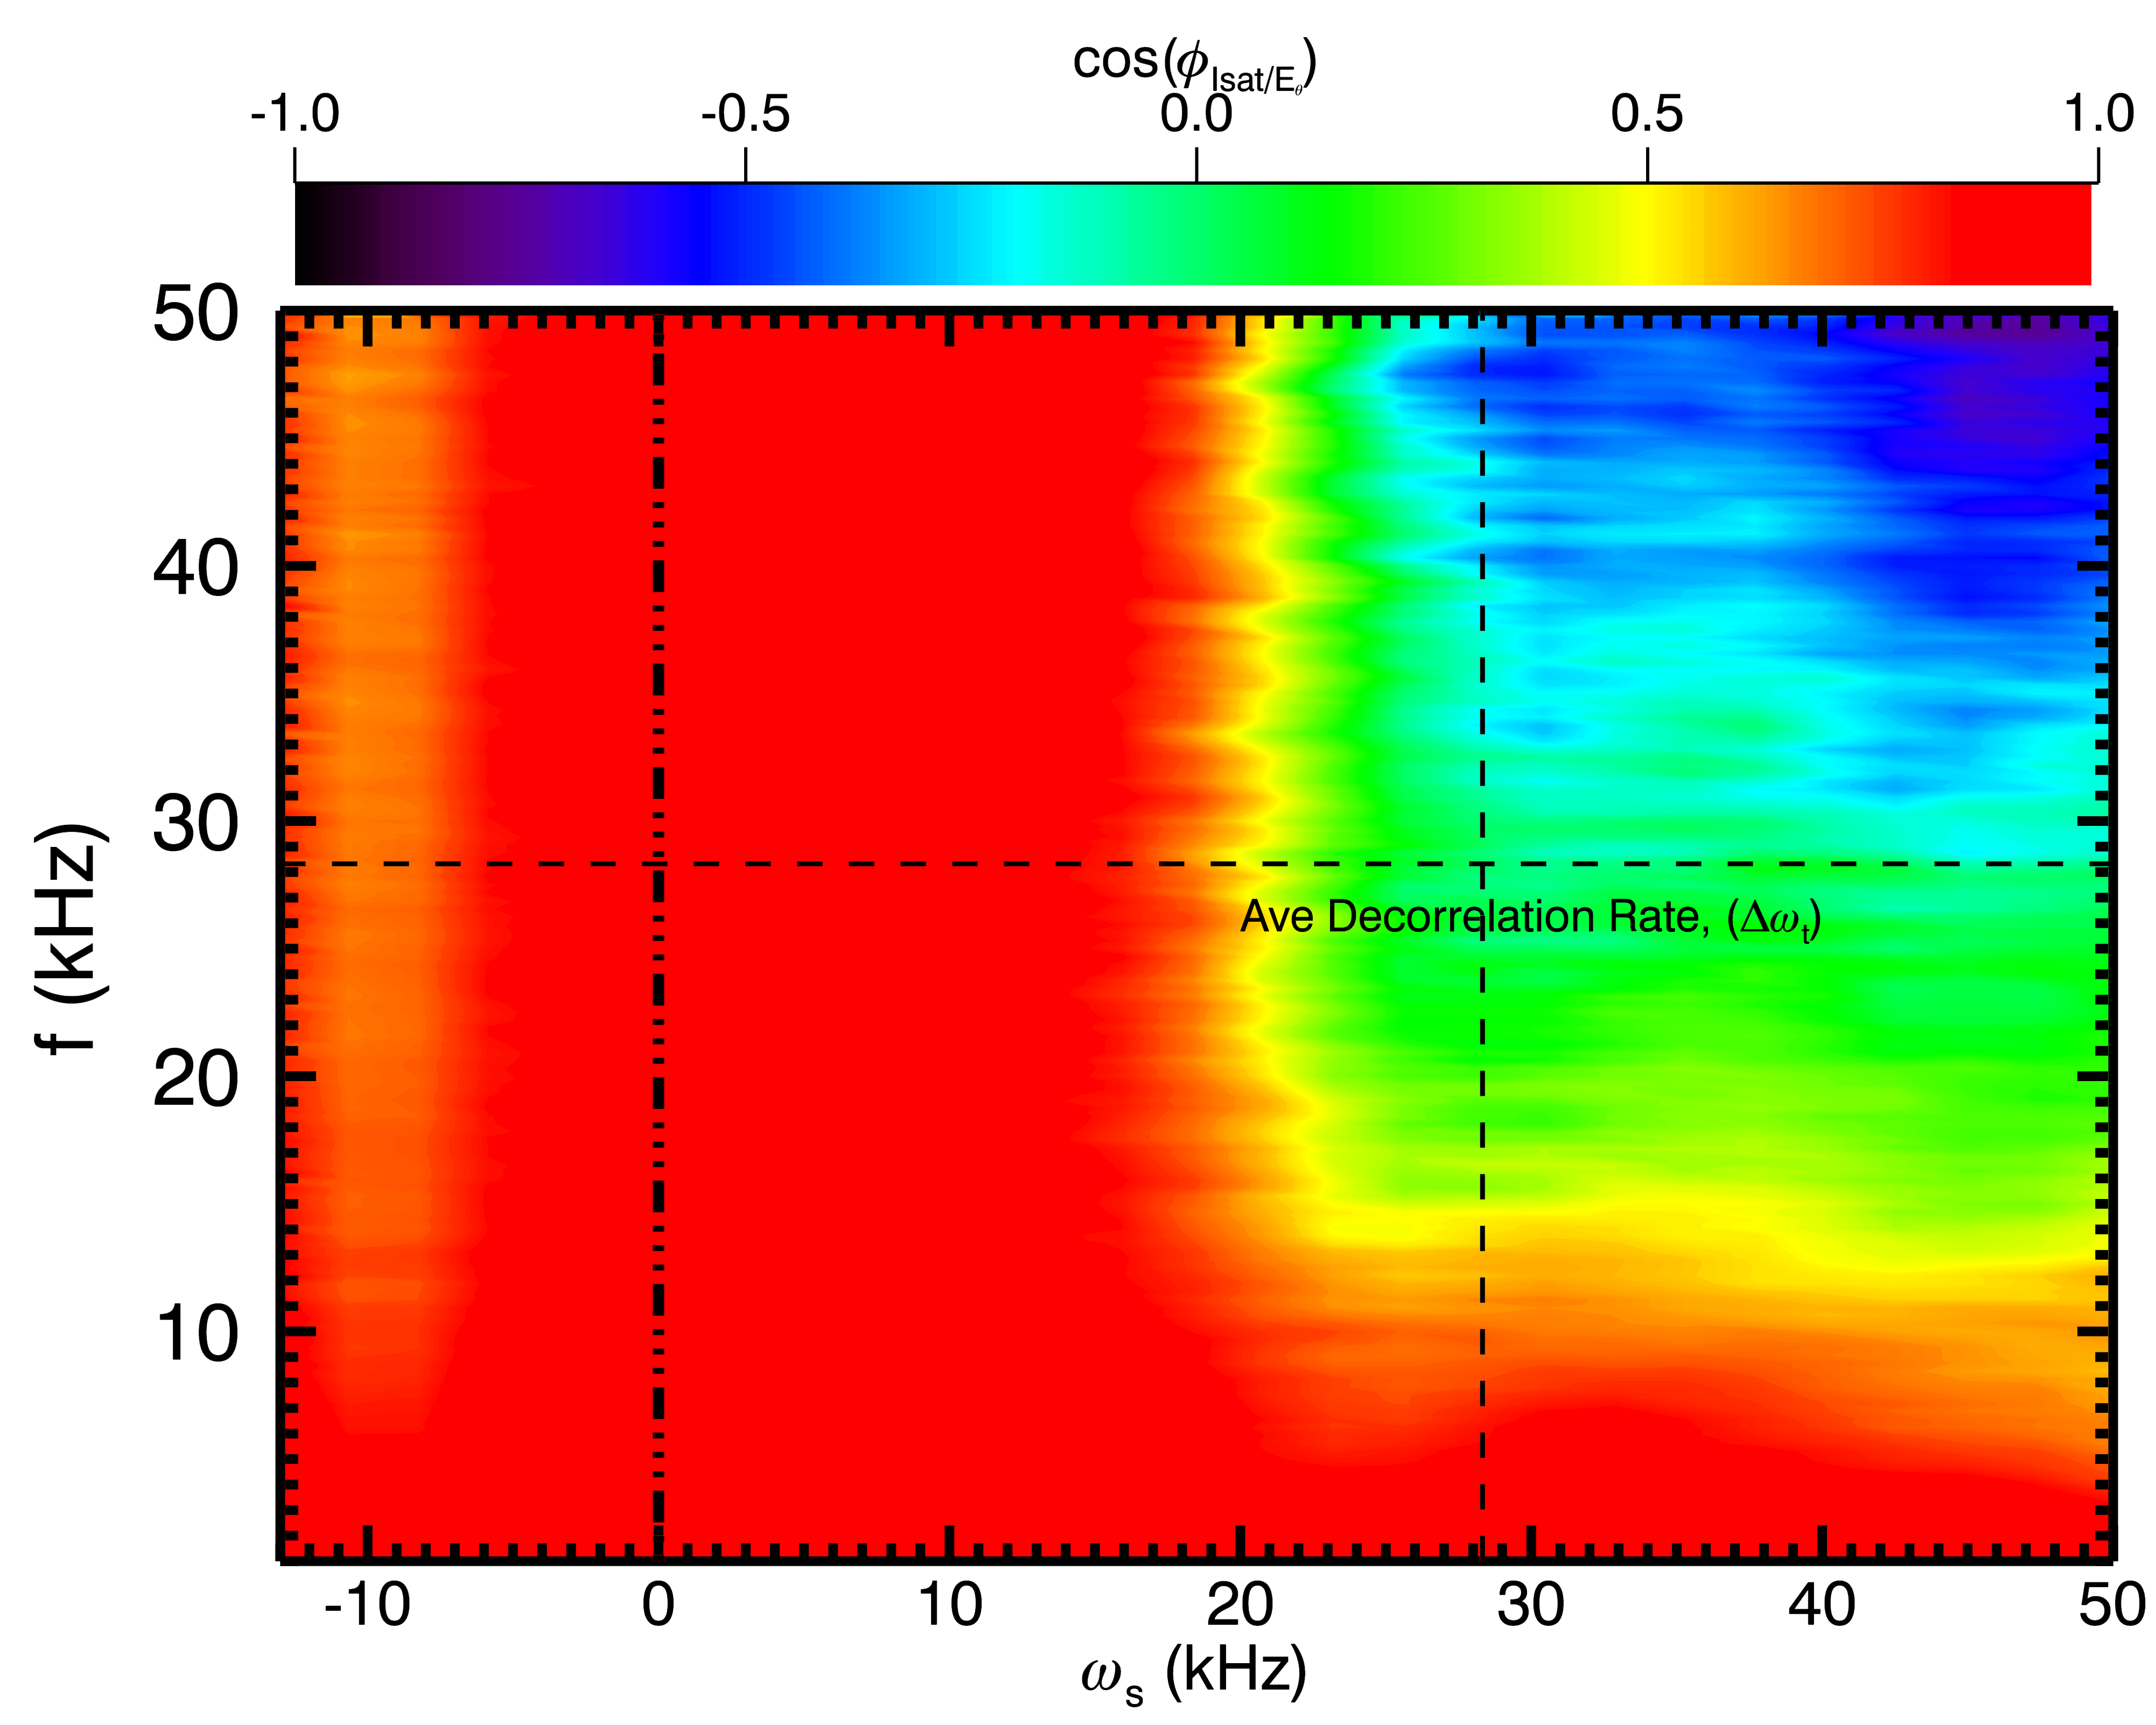
\includegraphics[width=8cm]{cpcontour.png}% Here is how to import EPS art
%\end{center}
%\caption{\label{fig:cpcontour} Contour plot isat/E-field crossphase versus shearing rate and frequency. Dashed lines show location of %decorrelation rate.}
%\end{figure}
%, shows no change from unity for all frequencies below 10kHz, but the exhibits sharp drops from 10kHz and above, starting consistently %at about 20kHz. 

Using a cross-correlation technique, we can show the modifications of turbulent structures by azimuthal shearing, specifically the shortening of the radial correlation length
Fig.~\ref{fig:radcorr}
\begin{figure}
\begin{center}
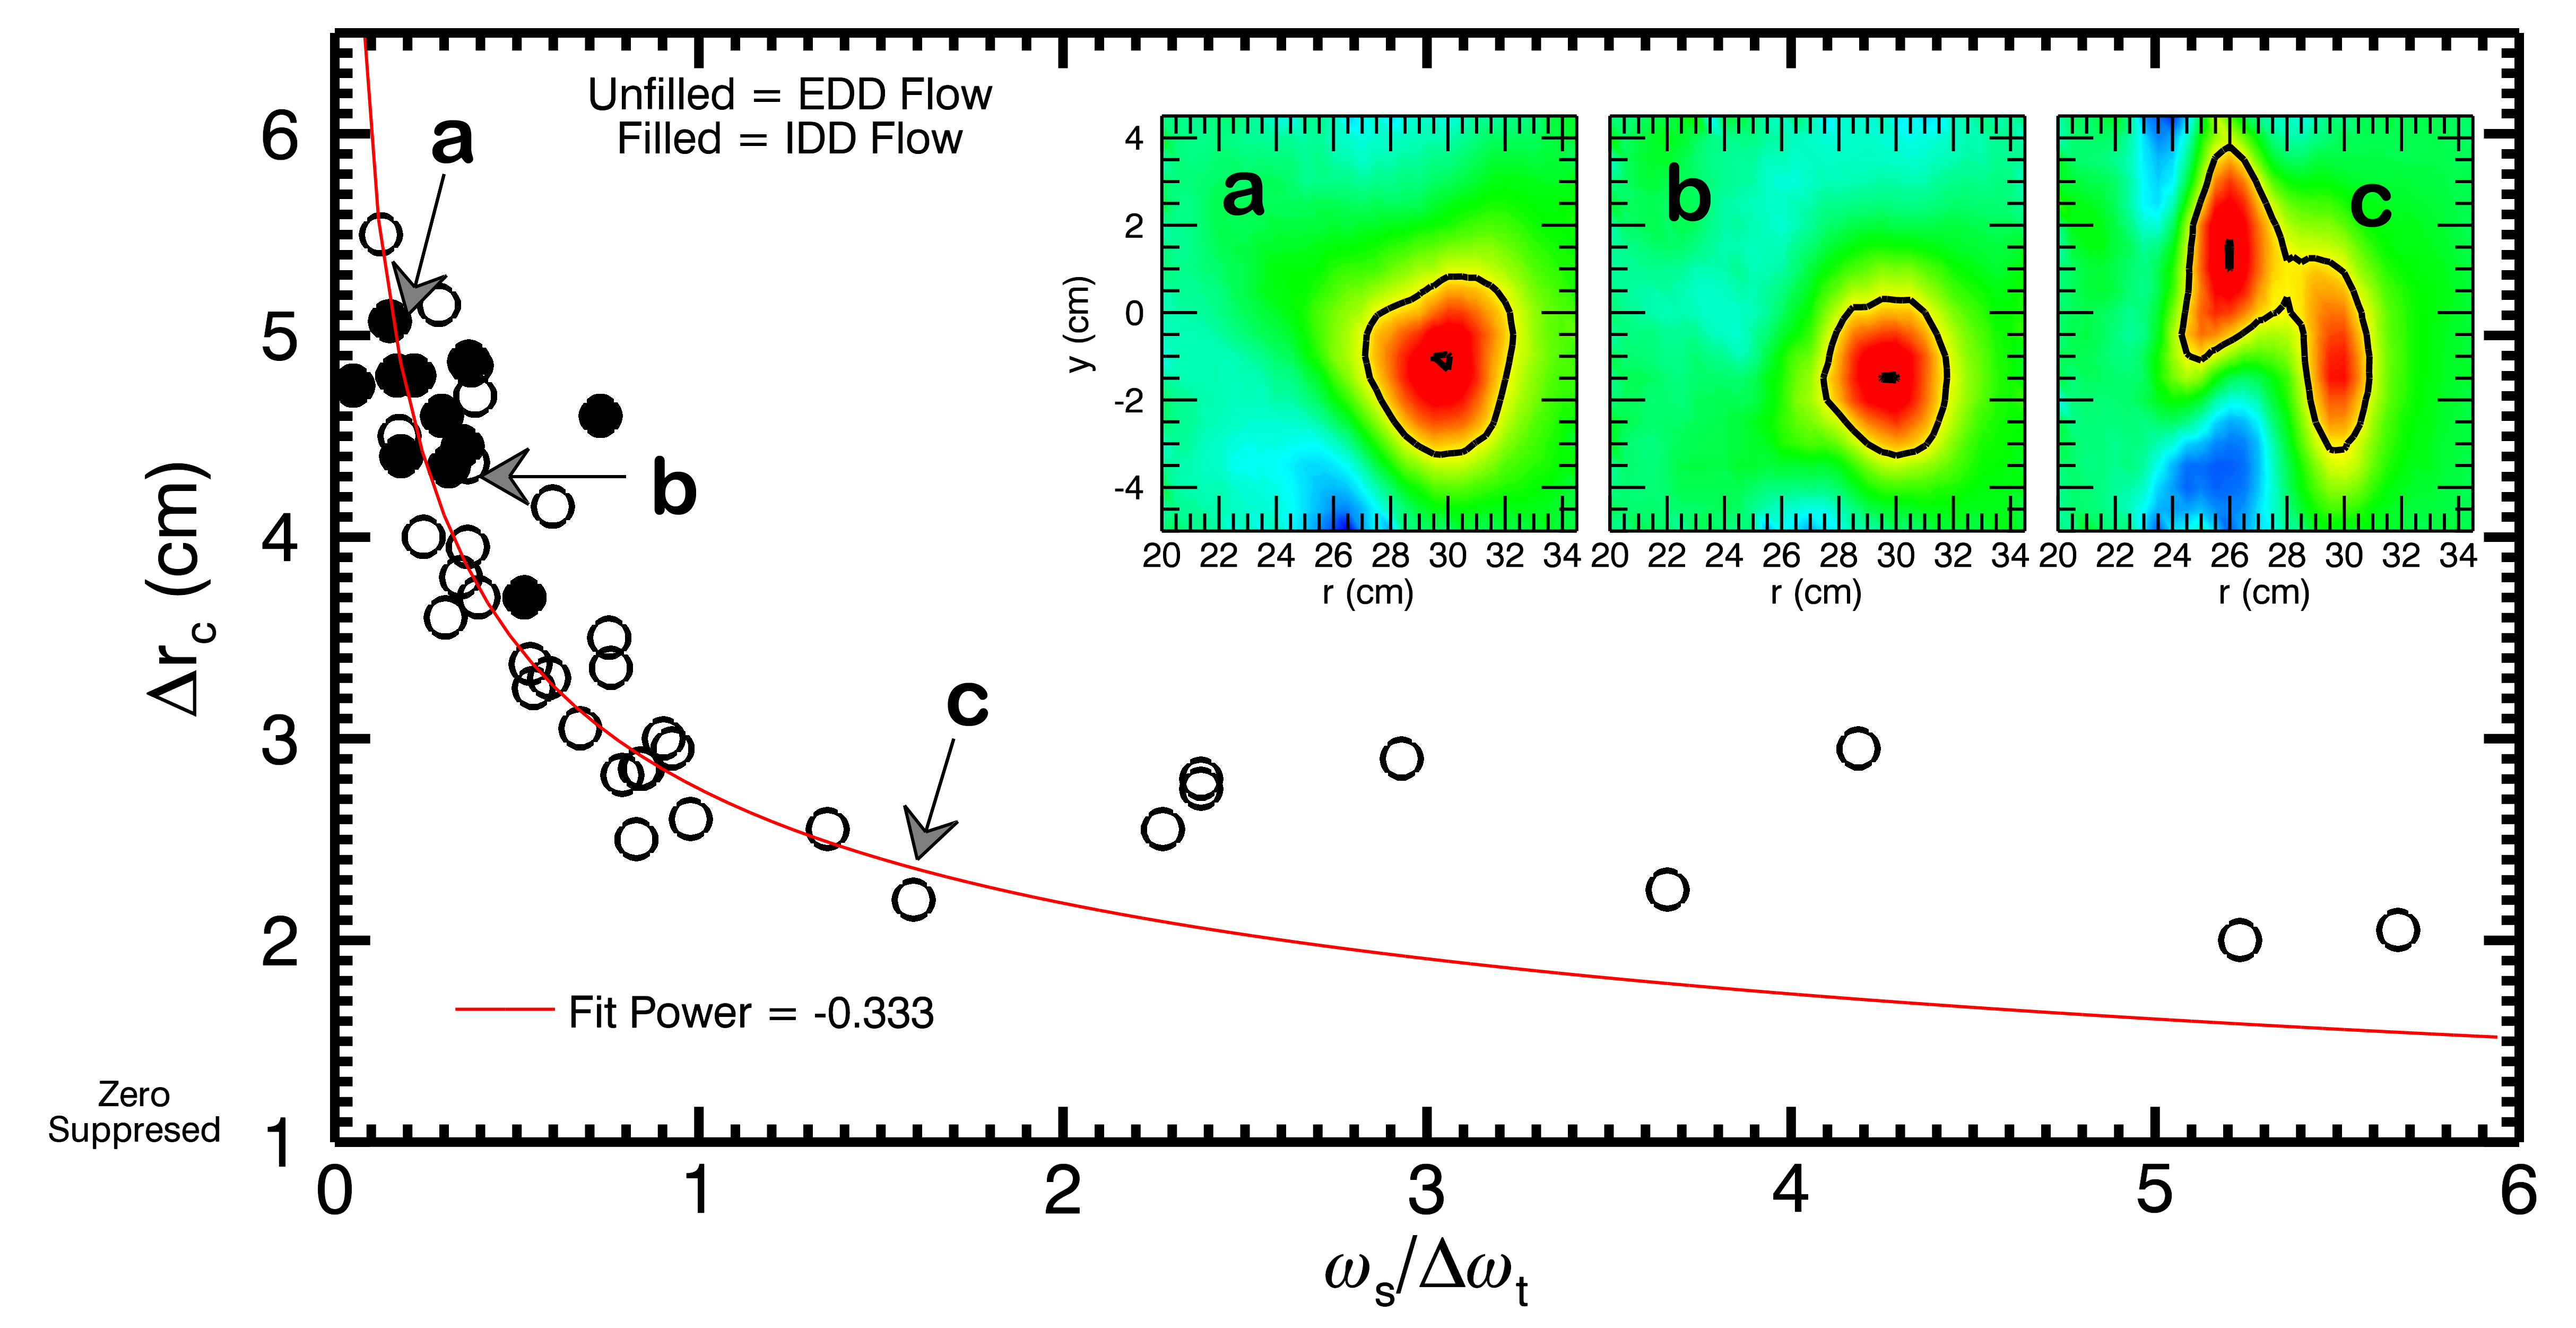
\includegraphics[width=8.5cm]{radcorr.pdf}% Here is how to import EPS art
\end{center}
\caption{\label{fig:radcorr} Measured radially correlation length with reference probe at 30cm and normalized to no-shear radial correlation length shows a decrease with flux that can be nearly fit to a power-law of -1/3. Inset shows 2D correlation length in azimuthal plane for low IDD flow shearing, no shear and high EDD flow shearing. The decrease in radial correlation can be seen as well as slight tilting depending on the direction of shear.}
\end{figure}
. The radially correlation length here is defined as the width of the contour plot to decrease to one-half its maximum value which occurs at the reference point, represented by the black curve in the inset of Fig.~\ref{fig:radcorr} and is normalized to the radial correlation length in the no-shear state. This correlation length decreases with shearing rate roughly following a power-law with $\alpha = -(1/3)$ indicating the sheared flow's ability to decrease the radial extend of a turbulent eddy. Like the flux and fluctuation data, the suppression begins with relatively little shearing. The correlation lengths can also be separated by frequency. High frequency correlation functions tend to be smaller than low frequency ones, though the normalized differences between the regimes is low. Note how IDD flow structures appear to grow someone wider with shear rather than EDD flow structures as show by the filled symbols. This may be due to contributions from a growing coherent mode with shear which is much more apparent and distinct in the EDD flow direction. This mode evidence in the correlation length can also be seen in the isat power spectrum
beginning to grow in the regime of shearing where it is nearly equal to the decorrelation rate. This mode also appears to grow linearly in frequency with shearing rate. In is unclear what the orgin of this mode is---whether it is a drift-wave or flute-like Kelvin Helmholtz or rotational interchange---as well as what effect is has on the turbulence or flux. 

%From these results, it is clear that outward radial particle flux is suppressed by a combination of turbulent fluctuations in density, %density/E-field phasing and density/E-field coherency which, consequently, induces a steepening of density gradients---i.e. confinement. %However, both processes appear to be most effective in different regimes. Fluctuations decreases seem to manifest in lower shearing %rate, lower frequencies while crossphase change is most apparent at higher shearing rate and higher frequencies. The reason for this %difference is still under examination, but could be a result of a relationship between of turbulent correlation length and shearing %scale length or perhaps due to the growth of new instabilities associated with flow and shearing including Kelvin-Helmholtz or %rotational interchange modes. Evidence for this last point exists in the isat fluctuation power of
%Fig.~\ref{fig:powercontour}
% where a coherent mode appears in the low frequency range at high shearing rate as well as the fact that high frequency isat %fluctuations actually increase with shearing rate. Whether this mode is connected to the effect of shearing on flux or just a separate %consequence of driving up the shearing and flow is unclear.

This letter presents the first detailed scan of shearing rate in a linear device and has shown a clear effect of particle flux and density confinement through both the mechanisms of turbulent fluctuation reduction and change in crossphase of saturated current and electric field. Moreover, the scan has allowed for comparison to theory predictions of the effect of shearing on both fluctuation power and crossphase. Fits of the data for both fluctuations and crossphase are consistent with the power law predictions proposed.

%\nocite{*}
\bibliography{FlowModPRL_bib}% Produces the bibliography via BibTeX.

\end{document}
%
% ****** End of file aipsamp.tex ******
